\documentclass[11pt]{article}

\usepackage{amsmath}
\usepackage{amssymb,latexsym}
\usepackage{amsthm}
\usepackage[spanish]{babel}
\usepackage[pdftex]{graphicx} % PDFLaTeX
\DeclareGraphicsExtensions{.png,.pdf,.jpg}
\usepackage{epsf}
\usepackage{graphicx}

\newtheorem{teorema}{Teorema}[section]
\newtheorem{lema}[teorema]{Lema}
\theoremstyle{definition}
\newtheorem{definicion}[teorema]{Definici\'on}
\newtheorem{problema}{Problema}
\newtheorem{ejemplo}{Ejemplo}

\renewcommand{\baselinestretch}{1.2}
\usepackage[bottom]{footmisc}  % places footnotes at page bottom
\usepackage[latin1]{inputenc}      %    tipo de codificacion del documento: applemac,

\usepackage{subfigure}
%\usepackage{hyperref}
%\usepackage[pdftitle={},pdfauthor={}, colorlinks=true, hyperindex=true, linkcolor=blue, pdfpagemode=UseOutlines, bookmarksopen=false, bookmarksnumbered=true, pdfstartview={FitH}]{hyperref} % %backref={page} para referencia de pagina
\spanishdecimal{.}
\usepackage{amssymb,amsmath,latexsym,amsfonts}
\usepackage{rotating}
\usepackage{indentfirst}        %
%\usepackage[]{showkeys}

\begin{document}

\title{C�LCULO PARA EL AN�LISIS ECON�MICO}
\author{\textbf{ESCUELA SUPERIOR DE ECONOM�A}}
\date{\large{M\'exico, D.F., 27 de Agosto de 2010}}
\def\contentsname{Contenido}

\newpage

\setcounter{page}{1}

\section{Derivadas}
\section{Optimizaci�n libre con una variable}
\section{C�lculo en varias variables}
\section{Optimizaci\'on libre y restringida en varias \\
         va\-ria\-bles}

\setcounter{page}{1}

\newpage
\section{Integral definida e indefinida}
\textbf{Introducci\'on}
\medskip

Hemos analizado como encontrar la derivada de una funci\'on. Sin
embargo, muchos problemas exigen como recuperar una funci\'on a
partir de su derivada conocida. Por ejemplo, supongamos que una
funci�n de costo marginal $C'(x)$ se da, es decir, se sabe c�mo
el costo est� cambiando de acuerdo a la cantidad producida $x$,
y estamos en busca de la correspondiente funci�n de costos $C(x)$.
Esta funci�n se puede encontrar por medio de la integraci�n,
que es lo contrario al proceso de diferenciaci�n. De manera m\'as general, queremos
encontrar una funci\'on $F$ a partir de su derivada $f$. Si tal
funci\'on $F$ existe, se llama  una antiderivada de $f$ y al
conjunto de todas las antiderivadas de $f$ se le llama la integral
indefinida de $f$.
\medskip

\textbf{Antiderivadas}

\begin{definicion}
Sea $f$ una funci\'on. Una antiderivada de $f$ es una funci\'on $F$
diferenciable tal que $F'(x) = f(x)$.
\end{definicion}

Si $F$ y $G$ son primitivas de $f$, entonces existe una constante
$c\in \Bbb{R}$, tal que:
\[
   F(x) = G(x) + c.
\]

\subsection{Integral indefinida.}

Las antiderivas de una funci\'on $f$ se les llama integrales
indefinidas de la funci\'on $f$  y se denotan:  Si $F$ es una
primitiva de $f$,
\[
   \int f(x) \, dx = F(x) + c
\]
donde $c \in \Bbb{R}$ es una constante arbitraria.

\vspace{.2cm}

\subsubsection{Reglas de integraci\'on.  }

 \vspace{.2cm}

\begin{enumerate}
    \item $\int ( c \cdot f(x)) \, dx = c \cdot \int f(x)\, dx$ \vspace{.2cm}
    \item $\int dx = x + c$  \vspace{.2cm}
    \item $\int x^{n}\, dx = \frac{x^{n + 1}}{n + 1} + c$, $n \ne -1$  \vspace{.2cm}
    \item $\int \frac{dx}{x} = ln |x| + c$  \vspace{.2cm}
    \item $\int e^{x} dx = e^{x} + c$  \vspace{.2cm}
    \item $\int sen\,x dx = -cos\, x + c $  \vspace{.2cm}
    \item $\int cos\,x dx = sen\, x + c$  \vspace{.2cm}
    \item $\int tg\,x \,dx = -\ln(cos\, x) + c$  \vspace{.2cm}
    \item $\int (f(x) + g(x))\, dx = \int\, f(x) dx  + \int g(x)\, dx$ \vspace{.2cm}
    \item $\int (f(x) - g(x))\, dx = \int\, f(x) dx  - \int g(x)\, dx$  \vspace{.2cm}
\end{enumerate}

\begin{ejemplo}
\begin{align*}
 \int(x^{2}-2x + 5) \, dx &= \int x^{2}  \,dx - \int 2x \,dx + \int 5  \,dx \\
                          &= \int x^{2} \,dx - 2\int x \,dx + 5 \int 1 \, dx \\
                          &= \frac{x^{3}}{3}- x^{2} + 5x + C.
\end{align*}
\end{ejemplo}

\subsection{T�cnicas de integraci\'on.}


\begin{itemize}
\item \textbf{Sustituci\'on o Cambio de Variable}:
\[
\int f(\mu) \, d \mu =  \int f(\varphi(t)) \cdot  \varphi'(t)  dt,
\]
donde $\mu = \varphi (x).$ \vspace{.2cm}

\begin{ejemplo}
Evaluar:
\[
    \int \frac{2x - 9}{\sqrt{x^{2} -9x  + 1 }} \, dx.
\]
\textbf{Soluci\'on:}


 Sean:
\begin{align*}
   u  &=  x^{2} - 9x + 1,  \\
  du  &= (2x - 9) \, dx.
\end{align*}
Entonces:
\begin{align*}
    \int \frac{2x - 9}{\sqrt{x^{2} -9x  + 1 }} \, dx &= \int
    \frac{du}{\sqrt{u}} \hspace{.7cm}           \\
   &= \int u^{-\frac{1}{2}} \, du \\
   &= \frac{  u^{(-1/2 ) + 1} }{(-1/2) + 1} + C \\
   &= 2u^{1/2} + C \\
   &= 2 \sqrt{x^{2} - 9x + 1} + C.
\end{align*}

\begin{ejemplo}
Evaluar:
\[
    \int \frac{2}{2x + 1} \, dx.
\]
\textbf{Soluci\'on}

Sean:
\begin{align*}
   u  &=  2x + 1 \\
  du  &= 2 \, dx. \\
\end{align*}
Entonces:
\begin{align*}
    \int \frac{2}{2x + 1 } \, dx &= \int
    \frac{du}{u} \hspace{.7cm}           \\
   &= \ln u \\
   &= \ln(2x + 1) + C
\end{align*}
\end{ejemplo}


\begin{ejemplo}
Evaluar:
\[
    \int e^{3x} \, dx.
\]
\textbf{Soluci\'on}


 Sean:
\begin{align*}
   u  &=  3x \\
  du  &= 3 \, dx. \\
\end{align*}
Entonces:
\begin{align*}
    \int e^{3x} \, dx &= \frac{1}{3} \int
    e^u \, du \hspace{.7cm}           \\
   &= \frac{e^u}{3}  \\
   &= \frac{e^{3x}}{3} + C
\end{align*}
\end{ejemplo}


\begin{ejemplo}
Evaluar:
\[
    \int sen(5x) \, dx.
\]
\textbf{Soluci\'on}


 Sean:
\begin{align*}
   u  &=  5x \\
  du  &= 5 \, dx. \\
\end{align*}
Entonces:
\begin{align*}
    \int sen(5x) \, dx &= \frac{1}{5} \int
    sen\, u \, du \hspace{.7cm}           \\
   &=  - \frac{\cos u}{5}  \\
   &= - \frac{\cos (5x)}{5} + C
\end{align*}
\end{ejemplo}


\begin{ejemplo}
Evaluar:
\[
    \int 3 \cos (4x) \, dx.
\]
\textbf{Soluci\'on}


 Sean:
\begin{align*}
   u  &=  4x \\
  du  &= 4 \, dx. \\
\end{align*}
Entonces:
\begin{align*}
    \int 3 \cos (4x) \, dx &= \frac{3}{4} \int
    \cos  u \, du \hspace{.7cm}           \\
   &=  \frac{3}{4} \cos u  \\
   &=  \frac{3}{4} \cos (4x) + C
\end{align*}
\end{ejemplo}


\end{ejemplo}


\item \textbf{Por Partes}: Sean $f, g$ funciones derivables. Entonces:
\[
\int f(x) \cdot g'(x) \, dx = f(x) \cdot g(x) - \int f'(x) \cdot
g(x) \, dx
\]
En ocasiones es m\'as f\'acil recordar la f\'ormula si la escribimos
en forma diferencial. Sea $u = f(x)$ y $v = g(x)$. Entonces $du =
f'(x) \, dx$ y $dv = g'(x) \, dx$. Utilizando la regla de
sustituci\'on, la f\'ormula de integraci\'on por partes se transforma
en:
\[
  \int u \,dv = uv - \int v \,du.
\]

\begin{ejemplo}
Evaluar la integral:
\[
   \int x e^x \, dx.
\]

Hacemos:
\begin{align*}
  u &= x,    &dv   &=  e^x \, dx, \\
 du &= dx,    &v    &= e^x\, dx.
 \notag
 \end{align*}
Entonces:
\[
  \int x e^x \, dx =x e^x  - \int e^x \, dx = x e^x +
  e^x = e^x (x -1) + C
\]
\end{ejemplo}

\begin{ejemplo}
Evaluar la integral:
\[
   \int x \cos x \, dx.
\]

Hacemos:
\begin{align*}
  u &= x,    &dv   &= \cos x \, dx, \\
 du &= dx,    &v    &= \sen x \, dx.
 \notag
 \end{align*}
Entonces:
\[
  \int x \cos  x \, dx = x \sen x - \int \sen x \, dx = x \sen x +
  \cos x + C.
\]
\end{ejemplo}
\end{itemize}

\begin{problema}
El costo marginal, como la funci\'on de las unidades producidas $x$,
esta dado por $C' = 10 + 40x -12x^2$. Hallar la funci�n de costo
total, sabiendo que \$100 es el costo fijo.

\vspace{.2cm}

\textbf{Soluci\'on al problema 17}

\vspace{.2cm}

Para determinar la funci\'on de costo total se calcula la integral
indefinida siguiente:

\begin{align*}
C(x) &= \int (10 + 40 x - 12x^2) \, dx \Rightarrow \\
C(x) &= 10 \int dx + 40 \int x \, dx  - 12 \int x^2 \, dx     \Rightarrow\\
C(x) &= 10x + 40 \frac{x^2}{2} - 12 \frac{x^3}{3} + k \Rightarrow\\
C(x) &= 10x + 20 x^2 - 4 x^3 + k
\end{align*}


Para determinar $k$ se utiliza el dato del costo fijo, vale decir:
si $x=0$, entonces $C(0)=100$.

\vspace{.2cm}

Por lo tanto: $C(0) = 10\cdot 0 + 20 \cdot 0^2 - 4 \cdot 0^3 + k
\Rightarrow   \quad 100 = k$

\vspace{.2cm}

Luego: $C(x) = 10x + 20x^2 - 4x^3 + 100$.
\end{problema}

\begin{problema}
Una empresa advierte que un incremento en el precio de \$1 provoca
una ca\'{\i}da en las ventas de 5 unidades. Adem\'as, la empresa
puede vender \$100 unidades a un precio de \$10 cada una. Encontrar
la funci\'on de demanda de la empresa.
\end{problema}
\vspace{.2cm}

\textbf{Soluci\'on al problema 18}

\vspace{.2cm}

Sea $q$ es la cantidad demandada con respecto al precio, entonces la
funci\'on de demanda es
\begin{align*}
\frac{dq}{dp} & =-5 \\
          dq  & =-5 \, dp \\
     \int dq  & =-5 \int dp \\
           q  & =-5p+k
\end{align*}

Entonces, para encontrar el valor de $k$, tenemos que
\begin{align*}
100 &= -5(10) + k \\
100 &= -50 + k \\
k &= 100 + 50 = 150
\end{align*}

Por lo tanto la funci\'on de demanda es $q =  -5p + 150$.

\begin{problema}
La propensi\'on marginal al consumo para M\'exico est\'a dada por:
\[
      \frac{dC}{dY} = \frac{3}{4} - \frac{1}{2 \sqrt{3Y}},
\]
donde el consumo $C$ es una funci\'on del ingreso nacional $Y$. En
esta caso $Y$ se expresa en miles de millones de pesos. Determinar
la funci\'on de consumo para M�xico si se sabe que el consumo es de
10 mil millones de pesos $(C=10)$ cuando $Y=12$.
\end{problema}

\textbf{Soluci\'on al problema 19:} Como la propensi\'on marginal al
consumo es $\frac{dC}{dY}$, tenemos que:
\begin{align*}
 C &= \int \frac{dC}{dY}  dY \\
   &=  \int \left( \frac{3}{4} - \frac{1}{2 \sqrt{3Y}} \right) \, dY \\
   &= \frac{3}{4}Y - \frac{1}{2} \int (3Y)^{-\frac{1}{2}} \, dY \\
   &= \frac{3}{4}Y - \left( \frac{1}{2}\right) \frac{1}{3}
  \int (3Y)^{-\frac{1}{2}}[3 \, dY] \\
  &= \frac{3}{4}Y - \frac{\sqrt{3Y}}{3} + C_1
\end{align*}
Como $C=10$ cuando $Y=12$, de la \'ultima ecuaci\'on se sigue que
$C_1=3$, por tanto la funci\'on de consumo es:
\[
   C = \frac{3}{4}Y - \frac{\sqrt{3Y}}{3} + 3.
\]

\newpage

\setcounter{page}{1}

\begin{center}
\textbf{TAREA 1: INTEGRAL INDEFINIDA}
\end{center}

Trabajo individual.

\vspace{.3cm}

\begin{enumerate}
\item[a)] Calcular las siguientes integrales:
\begin{align*}
1) & \int (x^3 + 2x^2 + x + 2) dx & \qquad
2) & \int (\sqrt{x} + \frac{1}{2 \sqrt{x}})\, dx & \qquad \\[.5cm]
3) & \int \frac{(\ln x)^2} {x} dx & \qquad
4) & \int \frac{ax^2}{\sqrt{x^3 + 8}}\, dx & \qquad \\[.5cm]
5) & \int \frac{5x}{x^2+1}\,dx  & \qquad
6) & \int \frac{1}{2x - 4}\, dx & \qquad \\[.5cm]
7) & \int \frac{1}{\cos^2 3x}\, dx & \qquad
8) & \int \frac{\cos x}{\sen^2 x}\, dx  & \qquad \\[.5cm]
9) & \int xe^{2x}\, dx  & \qquad
10) & \int \ln(x) dx
\end{align*}

\item [b)] El costo marginal, como la funci\'on de las unidades producidas $x$,
esta dado por $C' = 2 + 60x -5x^2$. Hallar la funci�n de costo
total, sabiendo que \$65 es el costo fijo.

\item [c)] La propensi\'on marginal al consumo en miles de millones est\'a dada
por:
\[
      \frac{dC}{dY} = \frac{7}{10} + \frac{0.2}{ \sqrt{Y}},
\]
Determinar la funci\'on de consumo si se sabe que el consumo es de 8
mil millones de pesos $(C=8)$ cuando $Y=0$.
\end{enumerate}

\newpage

\setcounter{page}{1}

\subsection{Integral definida}

\textbf{Introducci\'on}
\medskip

El \'area de la regi\'on  con una frontera curva puede ser
aproximada sumando \'areas de un conjunto de rect�ngulos. Al usar
m\'as rect�ngulos podemos aumentar la exactitud de la
aproximaci\'on. El proceso de l\'{\i}mite nos conduce a la
definici\'on de integral definida de una funci\'on en un intervalo
cerrado.
\medskip

La integral definida tiene muchas aplicaciones en estad\'{\i}stica y
econom\'{\i}a. Nos permite calcular rangos de cantidades de probabilidad y promedios de
consumo de energ\'{\i}a.


\subsection{Definici\'on de integral definida}
Sea $f$ una funci\'on continua no negativa en $[a, b]$. Entonces el
\'area $A$ de la regi\'on bajo la gr\'afica de $f$ es:
\[
 A = \lim_{n \to \infty} \, [f(x_1) + f(x_2) + \cdots + f(x_n) ]
 \,  \Delta x,
\]
donde $x_1,x_2,..., x_n$ son puntos arbitrarios en los $n$
subintervalos de $[a, b]$ del mismo ancho $ \Delta x =  \frac{b - a}{n}.$

\begin{definicion}
Sea $f$ una funci\'on continua definida en $[a, b]$. Si
\[
  \lim_{n \to \infty} \, [f(x_1) + f(x_2) + \cdots + f(x_n) ]
 \,  \Delta x,
\]
existe para todas las elecciones de puntos representativos
$x_1,x_2,...,x_n$ en los $n$ subintervalos de $[a, b]$ del mismo ancho
 $\Delta x = \frac{b - a}{n}$, entonces este l\'{\i}mite se llama
la \textbf{integral definida} de $f$ en $[a, b]$ y se le denota por
$\int_{a}^{b} f(x) dx$. As\'{\i} :
\[
  \int_{a}^{b} f(x) dx  = \lim_{n \to \infty} \,
[f(x_1) + f(x_2) + \cdots + f(x_n) ]
 \,  \Delta x.
\]
\end{definicion}


\textbf{Interpretaci\'on geom\'etrica de la integral definida}


\begin{itemize}
  \item Si $f$ es no negativa y continua en $[a, b]$, entonces:
 \[
\int_{a}^{b} f(x) dx
\]
es el \'area de la regi\'on bajo la gr\'afica de $f$ en el intervalo
$[a, b]$. \vspace{.3cm}
  \item  Si $f$ es continua en $[a, b]$, entonces:
 \[
\int_{a}^{b} f(x) dx
 \]
es el \'area de la regi\'on por arriba del intervalo $[a, b]$ menos el
\'area de la regi\'on por debajo de $[a, b]$.
\end{itemize}

\begin{ejemplo}
Trazar la gr\'afica y hallar el �rea de la regi�n acotada por debajo
de la gr�fica de la funci�n $f$ y arriba del eje $x$ donde:
\[
f(x) = -x^2+4
\]

\textbf{Soluci�n}
\medskip

Igualando a cero la $f$ obtenemos los puntos de intersecci\'on con
el eje $x$
\begin{align*}
-x^{2}+4 &=0\\
4 &=x^{2} \\
x^{2} &=4 \\
x &=\pm2
\end{align*}
Los puntos de intersecci�n son $-2$ y $2$, entonces el \'area entre
esta gr�fica y el eje $x$ es (ver figura 25):
\begin{align*}
   \int_{-2}^{2} f(x) dx  &= \int_{-2}^{2} [-x^2 + 4] dx \\
   &= (-\frac{x^3}{3} + 4x) \Bigg|_{-2}^{2} \\
   & = (-\frac{2^{3}}{3}+4(2)) - (-\frac{(-2)^{3}}{3}+4(-2)) \\
   &= \frac{32}{3}.
\end{align*}
\end{ejemplo}

\begin{figure}[h]
\begin{center}
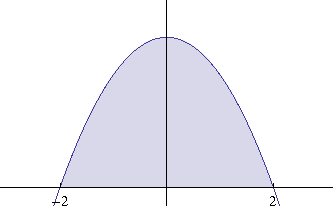
\includegraphics[width= 0.7 \textwidth,height=0.29
\textheight]{unid1graf33.pdf}
\end{center}
\caption{$f(x) = -x^2+4$}\label{Figura23}
\end{figure}

\newpage

\begin{ejemplo}
En estad\'{\i}stica, una funci\'on de densidad (de probabilidad) $f$
de una va\-ria\-ble $x$, donde $x$ toma todos los valores en el intevalo $[a, b]$,
tiene las siguientes propiedades:

 \vspace{.2cm}

\begin{enumerate}
   \item $f(x) \geq 0 .$  \vspace{.2cm}
   \item $ \int_{a}^{b} f(x)  dx = 1.$  \vspace{.2cm}

 Si $f$ es una funci\'on de densidad de probabilidad continua, la media $\mu$ de $f$ en el intervalo $[a,b]$
  est\'a definida por:
  \[
   \mu = \int_{a}^{b} [x \cdot f(x)] dx,
  \]
y la varianza $\sigma^2$ est\'a dada por
\[
 \sigma^2 =\int_{a}^{b}   (x - \mu)^2 f(x) dx,
\]

   La probabilidad de que $x$ tome un valor entre $c$ y $d$, lo
   cual se escribe $P(c \leq x \leq d)$,  donde
   $a \leq c \leq x \leq d \leq b,$ se representa por el \'area de la
   regi\'on limitada por la gr\'afica de $f$ y el eje $x$ entre $x =
   c$ y $x = d$. Por tanto:
\[
   P(c \leq x \leq d)  =  \int_{a}^{b} f(x) \, dx.
\]
\end{enumerate}


\vspace{.2cm}

La funci\'on  $f(x) = 6 (x - x^{2})$, donde $0 \leq x
\leq 1$, satisface que es una funci\'on de densidad, por:
\[
f(x) = 6(x- x^2) =6x(1-x) \geq 0
\]
en $[0,1]$ ya que $6x \geq 0 $ si $x \geq 0 $ y $1- x \geq 0$ si $ x \leq 1$, lo cual se cumple pues $x \in [0,1]$, ademas:
\[
\int_{0}^{1} 6 (x- x^2) dx = 6\int_{0}^{1} ( x- x^2) dx =6 (\frac{x^2}{2}- \frac{x^3}{3}) \Bigr|_{0}^{1} = 6 (\frac{1}{2}- \frac{1}{3} )=6( \frac{1}{6})  =1
\]
\medskip
\,\,\,\,\,\,\,con media $\mu$
  \begin{align*}
   \mu &= \int_{0}^{1} [x \cdot f(x)] dx = \mu = 6 \int_{0}^{1} [x (x-x^2)  ] dx \\
   & = 6 \int_{0}^{1} [x^2 - x^3] dx = 6 (\frac{x^3}{3}- \frac{x^4}{4}) \Bigr|_{0}^{1} = 6 (\frac{1}{3}- \frac{1}{4} )=6( \frac{1}{12})= \frac{1}{2}
  \end{align*}

y varianza $\sigma^2$
\begin{align*}
 \sigma^2  &=\int_{0}^{1}   (x - \frac{1}{2})^2 f(x) dx = \int_{0}^{1}   (x^2 -x +\frac{1}{4}) (6 (x- x^2)) dx  \\
& = 6 \int_{0}^{1}   (x^2 -x + \frac{1}{4}) (x- x^2) dx  = 6 \int_{0}^{1}   (x^3 -x^2 + \frac{x}{4}- x^4  + x^3 -\frac{x^2}{4}) \\
 &= 6 (-\frac{x^5}{5} + \frac{x^4}{2}-\frac{5x^3}{3} + \frac{x^2}{8}) \Bigr|_{0}^{1} \\
 &= 6(-\frac{1}{5} + \frac{1}{2} -\frac{5}{12} + \frac{1}{8}) = \frac{1}{20}
\end{align*}


 \vspace{.2cm}

Para esta funci\'on, podemos encontrar las siguientes probabilidades:
\begin{enumerate}
\item[a)] $P( 0 \leq x \leq \frac{1}{4})$.
\end{enumerate}

\vspace{.2cm}

\textbf{Soluci\'on}:  Por la propiedad 3:
\begin{align*}
   P(0 \leq x \leq \frac{1}{4}) &= \int_{0}^{\frac{1}{4}} 6(x - x^{2})
   \, dx  \\
   &=  6  \,  \int_{0}^{\frac{1}{4}} (x - x^{2})   \, dx  \\
   &= 6 \left( \frac{x^{2}}{2} - \frac{x^{3}}{3} \right )
   \Bigr|_{0}^{\frac{1}{4}} \\
   &= (3x^{2} -  2 x^{3}) \Bigr|_{0}^{ \frac{1}{4}} \\
   &= \frac{5}{32}.
\end{align*}

\item[b)] $P( x \geq \frac{1}{2})$.

\vspace{.2cm}

\textbf{Soluci\'on}:
\begin{align*}
   P(x \geq \frac{1}{2}) &= \int_{\frac{1}{2}}^{1} 6(x - x^{2})
   \, dx  \\
   &=  6  \,  \int_{\frac{1}{2}}^{1} (x - x^{2})   \, dx  \\
   &= 6 \left( \frac{x^{2}}{2} - \frac{x^{3}}{3} \right )
   \Bigr|_{\frac{1}{2}}^{1} \\
   &= (3x^{2} -  2 x^{3}) \Bigr|_{\frac{1}{2}}^{1} \\
   &= \frac{1}{2}.
\end{align*}
\end{ejemplo}

\newpage

\subsection{\'Area entre dos curvas}

Sean $f$ y $g$ funciones continuas tales que $f(x) \geq g(x)$ en el intervalo $[a, b]$. Entonces
el \'area de la regi\'on acotada por arriba por $y = f(x)$ y por abajo por  $y = g(x)$ en $[a, b]$
est\'a dada por:
\[
 \int_{a}^{b}[f(x) - g(x)] \, dx.
\]

\begin{ejemplo}
Trazar la gr\'afica de las funciones $f$ y $g$ y determine el \'area
de la regi\'on encerrada entre estas gr\'aficas donde:

\[
f(x) = x^2 \, \text{y} \, g(x) = x^3
\]

\textbf{Soluci�n}
\medskip

Igualando ambas funciones $f$ y $g$ obtenemos los puntos de
intersecci\'on entre las gr\'aficas de las funciones
\begin{align*}
x^{2} &= x^{3}\\
x^{2}-x^{3} &=0 \\
x^{2}(1-x) &=0 \\
x^{2}&=0 \\
(1-x) &=0
\end{align*}

Los puntos de intersecci�n son $(0,0)$ y $(1,1)$, entonces el \'area
entre estas graficas es (ver figura 26):
\begin{align*}
   \int_{0}^{1} [f(x) - g(x)] dx  &= \int_{0}^{1} [x^2 - x^3] dx \\
   &= (\frac{x^3}{3} - \frac{x^4}{4}) \Bigg|_{0}^{1} \\
   & = \frac{1}{3} - \frac{1}{4} \\
   &= \frac{1}{12}.
\end{align*}
\end{ejemplo}

\begin{figure}[h]
\begin{center}
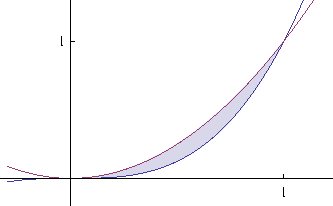
\includegraphics[width= 0.7 \textwidth,height=0.29
\textheight]{unid1graf31.pdf}
\end{center}
\caption{$f(x) = x^2$ y $g(x) = x^3$}\label{Figura23}
\end{figure}

\begin{ejemplo}
Una curva de Lorenz $y=L(x)$ se utiliza para estudiar las distribuciones de ingresos. Si $x$ es el porcentaje acumulativo de receptores de ingresos, ordenados de m\'as pobres a m\'as ricos, y $y$ es el porcentaje acumulativo de ingresos, entonces la igualdad de la distribuci\'on de ingresos est\'a dada por la recta $y= x$, donde $x$ y $y$ se expresan como decimales. Por ejemplo, 10 \% de la gente recibe 10 \% de los ingresos totales, 20 \% de la gente recibe 20 \% de los ingresos, etc\'etera.
\medskip

Si $y=L(x)$ es la ecuaci\'on de una curva de Lorentz, entonces la desigualdad en la distribuci\'on de riqueza correspondiente se mide mediante el \'{\i}ndice  de Gini $G$, cuya formula esta dada por
\[
G = 2 \int_{0}^{1}[x - L(x)] dx
\]
El \'indice de Gini siempre se situa entre 0 y 1. Un \'indice de 0 corresponde a una igualdad completa. Cuanto m\'as peque\~{n}o sea el \'{\i}ndice, m\'as equitativa ser\'a la distribuci\'on de la riqueza; cuanto m\'as grande sea el \'{\i}ndice, m\'as riqueza estar\'a concentrada en pocas manos. Ver figura 27.
\medskip

\begin{figure}[h]
\begin{center}
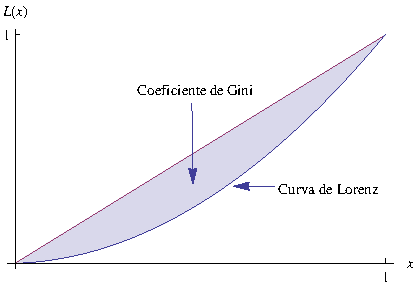
\includegraphics[width= 0.6 \textwidth,height=0.29
\textheight]{Gini1.pdf}
\end{center}
\caption{Curva de Lorenz y coeficiente de Gini}\label{Figura23}
\end{figure}

Suponga que la distribuci\'on real esta dada por la curva de Lorenz definida por
\[
 L(x) = \frac{20}{21}x^2 + \frac{1}{21}x.
\]
\begin{align*}
G   &= 2 \int_{0}^{1}[x - L(x)] dx = 2 \int_{0}^{1} (x- (\frac{20}{21}x^2 + \frac{1}{21}x)) dx \\
&=2 \int_{0}^{1} (-\frac{20}{21}x^2 + \frac{20}{21}x) dx =  2 (-\frac{20}{63}x^3 + \frac{20}{42}x^2)\Bigg|_{0}^{1} \\
& = 2(-\frac{20}{63} + \frac{20}{42}) =0.3
\end{align*}
Por lo tanto, el valor (0,3 , 0,1) significa que el 30\% de la poblaci�n posee el 10\% de la riqueza total en la sociedad. Ver figura 28.
\end{ejemplo}
\begin{figure}[h]
\begin{center}
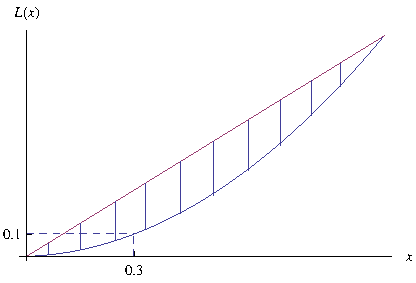
\includegraphics[width= 0.6 \textwidth,height=0.29
\textheight]{Gini.pdf}
\caption{$\frac{20}{21}x^2+\frac{1}{21}x$}\label{Figura23}
\end{center}
\end{figure}

\begin{problema}
La funci\'on de demanda para un producto es:
\[
   p = D(q) = 100- 0.05q,
\]
donde $p$  es el precio por unidad (en pesos) de $q$ unidades. La
funci\'on de oferta es:
\[
    p = S(q) = 10 + 0.1q.
\]
Determinar el excedente de los consumidores y de los productores,
bajo equilibrio de mercado.
\end{problema}

Supongamos que el mercado para un producto est\'a en equilibrio y que
$(q_0,p_0)$ es el punto de equilibrio (el punto de intersecci\'on de
las curvas de demanda y oferta para el producto). El excedente de
los consumidores, y se abrevia EC, corresponde al \'area
entre $q = 0$ y $q = q_0$, limitada por arriba por
la curva de demanda y abajo por la recta $p =p_0$. Entonces,
\[
 \text{EC} = \int_{0}^{q_0} [ f(q) - p_0] \,dq,
\]
donde $f$ es la funci\'on  de demanda. El excedente de los
productores, y se abrevia EP, corresponde al \'area, entre $q = 0$ y
$q =q_0$. limitada por arriba por la recta $p = p_0$ y abajo por la
curva de oferta. Entonces:
\[
 \text{EP} = \int_{0}^{q_0} [ p_0 - g(q)] \,dq,
\]
donde $g$ es la funci\'on de oferta.

\vspace{.2cm}

\textbf{Soluci\'on del problema 20:} Primero debemos encontrar el
punto de equilibrio $(p_0,q_0)$ resolviendo el siguiente sistema de
ecuaciones:
\begin{align*}
   p &=  100 - 0.05q \\
   p &=  10 + 0.1q.
\end{align*}
Por el m\'etodo de igualaci\'on, tenemos que:
\begin{align*}
  10 + 0.1q &= 100- 0.05q,\\
     0.15q &= 90, \\
      q &= 600.
\end{align*}
Cuando $q=600$, $p = 10 + 0.1(600) = 70.$ As\'{\i}, $q_0 =600$ y
$p_0=70$. El excedente de los consumidores es:
\begin{align*}
 \text{EC} &= \int_{0}^{q_0} [ f(q) - p_0] \,dq, \\
           &= \int_{0}^{600} [100-0.05q - 70] \,dq, \\
           &= \left(30q - 0.05 \,  \frac{q^{2}}{2} \right)
           \Bigr|_{0}^{600} \\
           &= 9000.
\end{align*}
 El excedente de los productores es:
\begin{align*}
 \text{EP} &= \int_{0}^{q_0} [ p_0 - g(q)] \,dq, \\
           &= \int_{0}^{600} [70 - (10 + 0.1q)] \,dq, \\
           &= \left(60q - 0.1 \,  \frac{q^{2}}{2} \right)
           \Bigr|_{0}^{600} \\
            &= 18000.
\end{align*}
Por tanto, el excedente de los consumidores es de \$9,000 y el de
los pro\-ducto\-res es de \$18,000.

\subsection{Integral impropia}

La definici\'on de la integral definida $\int_{a}^{b} f(x) \, dx$
requiere que el intervalo de integraci\'on $a \leq x \leq b$ este
acotado, pero en ciertas aplicaciones  es \'util considerar
integrales sobre intervalos no acotados como $x \geq a.$ A este tipo
de integrales se les llaman \textbf{integrales impropias}.

\begin{definicion}
(\textbf{La integral impropia}). Si $f(x)$ es continua para $x \geq
a$, entonces:
\[
   \int_{a}^{\infty} f(x) \, dx = \lim\limits_{N \to  \infty}
   \int_{a}^{N} f(x) \,dx
\]
Si el l\'{\i}mite existe, se dice que la integral \textbf{converge}
al valor del l\'{\i}mite. Si no existe el l\'{\i}mite, se dice que
la integral impropia \textbf{diverge}.
\end{definicion}


\begin{ejemplo}
Evalu\'e  o demuestre que converge la integral impropia:
\[
    \int_{1}^{\infty} \frac{1}{x^2} \, dx
\]
\textbf{Soluci\'on:} Primero calcule la integral de $1$ a $N$ y
luego haga que $N$ tienda al infinito. Contin\'ue su trabajo de este
modo:
\[
\int_{1}^{\infty} \frac{1}{x^2} \, dx  = \lim\limits_{N \to \infty}
\int_{1}^{N} \frac{1}{x^2}\,dx = \lim\limits_{N \to  \infty} \left(-
\frac{1}{x}\,  \Big|_{1}^{N} \right) = \lim\limits_{N \to  \infty}
\left(-\frac{1}{N} + 1 \right)=1
\]
\end{ejemplo}

\begin{ejemplo}
Evalu\'e o demuestre que diverge la integral impropia:
\[
    \int_{1}^{\infty} \frac{1}{\sqrt{x}} \, dx
\]
\textbf{Soluci\'on:} Primero calcule la integral de $1$ a $N$ y
luego haga que $N$ tienda al infinito. Contin\'ue su trabajo de este
modo:
\[
\int_{1}^{\infty} \frac{1}{\sqrt{x}} \, dx  = \lim\limits_{N \to \infty}
\int_{1}^{N}  x^{-1/2} \,dx = \lim\limits_{N \to  \infty}  \left(2x^{1/2}\,  \Big|_{1}^{N} \right)
= \lim\limits_{N \to  \infty}
\left(2 \sqrt{x} - 1\right)=\infty 
\]
Por lo tanto la integral impropia diverge.
\end{ejemplo}

\textbf{Un test de comparaci\'on para la convergencia}
\medskip

El siguiente test de convergencia de integrales suele ser \'util por
que no requiere el c\'alculo de la integral.

\begin{teorema}
\label{convergencia} ( \textbf{Un test de comparaci\'on para la
convergencia}) Su\-pon\-ga\-mos que $f$ y $g$ son continuas para
toda $x \geq a$ y que
\[
    \mid  f(x)  \mid \leq  g(x)   \quad (\text{para toda} x \leq a)
\]
\end{teorema}

Si $\int_{a}^{\infty} g(x) \, dx$ converge, entonces
$\int_{a}^{\infty} f(x) \, dx $ y
\[
\left| \int_{a}^{\infty} f(x) \, dx \right| \leq \int_{a}^{\infty}
g(x) \, dx
\]

\begin{ejemplo}
Para todo $x \geq 1$, se tiene $0 \leq e^{-x^2} \leq e^{-x}$. Como
$\int_{1}^{\infty} e^{-x} \, dx$ converge, por el Teorema
(\ref{convergencia}), la integral $\int_{1}^{\infty} e^{-x^2} \, dx$
tambi\'en converge.
\end{ejemplo}

\begin{ejemplo}
En la teor\'{\i}a de crecimiento econ\'omico aparecen frecuentemente
integrales de la forma
\begin{equation}
\label{convergencia1}
   \int_{t_0}^{\infty} U(c(t)) e^{-\alpha t} \, dt
\end{equation}
En la expresi\'on, $c(t)$ designa el consumo en el momento $t$, $U$
es la funci\'on de utilidad instant\'anea y $\alpha$ es una tasa
positiva de descuento. Supongamos que existen n\'umeros $M$ y
$\beta$, con $\beta \leq \alpha$, tales que
\begin{equation}
\label{convergencia2}
     \mid U(c(t)) \mid  \leq M e^{\beta t}
\end{equation}
pata todo $t \geq t_0$ y para todo nivel posible de consumo $c(t)$ en el tiempo $t$. As\'{\i}, el valor absoluto de la utilidad de consumo crece a  una tasa menor  que la de descuento $\alpha$. Probar que, entonces (\ref{convergencia1})  converge. \\

\vspace{.2cm}

Soluci\'on: De (\ref{convergencia2}) obtenemos
\[
     \mid U(c(t)) e^{-\alpha t} \mid  \leq M e^{-(\alpha- \beta) t} \quad (\text{parea todo} t \geq t_0)
\]
Adem\'as,
\[
   \int_{t_0}^{T} M e^{(\alpha - \beta) t} \, dt = \bigg|_{t_0}^{T} \frac{-M}{\alpha - \beta} e^{(\alpha - \beta)t}
   = \frac{M}{\alpha - \beta} \left[e^{-(\alpha -\beta)t_0} - e^{-(\alpha - \beta)T}  \right]
\]

Como $\alpha - \beta > 0$, la \'ultima expresi\'on tiende a $[ M /
(\alpha - \beta)] e^{-(\alpha - \beta) t_0}$ cuando $T \to \infty$.
Se deduce del Teorema (\ref{convergencia}) que
(\ref{convergencia1}) converge.
\end{ejemplo}

\newpage

\setcounter{page}{1}

\begin{center}
\textbf{TAREA 2: INTEGRAL DEFINIDA}
\end{center}

\vspace{.3cm}

Trabajo individual

\vspace{.2cm}

\begin{enumerate}
\item Trazar la gr\'afica y hallar el \'area de la regi\'on acotada por
debajo de la gr\'afica de la funci\'on $f$ y por arriba del eje $x$,
de $x = a$ a $x = b$, donde:
\begin{enumerate}
   \item[a)] $f(x) = 2x-x^{2}$ ;\, $a = 0, b = 2.$
   \item[b)] $f(x) = 4-x^{2}$;\,  $a = -2, b= 2.$
   \item[c)] $f(x) = x e^{-x^{2}}$;\, $a= 0, b = 3.$
\end{enumerate}
\item  Trazar la gr\'aficas de las funciones $f$ y $g$ y determine el \'area de la region encerrada
entre estas gr\'aficas donde:
\begin{enumerate}
   \item[a)] $f(x) = 4- x^{2}$ y $g(x) = x^{2}$.
   \item[b)] $f(x) = x+2$ y $g(x) = x^{2}$.
   \item[c)] $f(x) = 5x -x^{2}$ y $g(x) = x $.
\end{enumerate}
\item C\'alcule el \'{\i}ndice de Gini para las siguientes curvas de Lorenz e interprete:
\begin{enumerate}
\item[a)] $L(x) = \frac{3}{5}x^2 + \frac{2}{5}x$.
\item[b)] $L(x) = 0.8 x^2 + 0.2 x$.
\end{enumerate}
\item Encuentre el excedente de los consumidores y de los productores bajo
equilibrio de mercado de las siguientes funciones de demanda y
oferta
\begin{enumerate}
   \item[a)] $D(q)=16-q^{2}$ y $S(q)=4+q$.
   \item[b)] $D(q)=14-q^{2}$ y $S(q)=2q^{2}+2$.
\end{enumerate}
\item Demuestre la convergencia o divergencia de las siguientes integrales:
\begin{align*}
  a)\int_{1}^{\infty} \frac{1}{x^3} dx  && b) \int_{1}^{\infty} x^{-3/2} dx && c) \int_{0}^{\infty} \lambda e^{-\lambda x} dx
\end{align*}
\end{enumerate}


\newpage

\setcounter{page}{1}

\end{document}
